\documentclass{beamer}
\usepackage{fontspec}
\usepackage{graphicx}
\usepackage{hyperref}
\usepackage{xcolor}
\usepackage{booktabs}
\usepackage{tikz}

% Set the theme
\usetheme{Madrid}
\usecolortheme{default}

% Colors
\definecolor{mainblue}{RGB}{31, 119, 180}
\definecolor{accentorange}{RGB}{255, 127, 14}
\setbeamercolor{title}{fg=white, bg=mainblue}
\setbeamercolor{frametitle}{fg=mainblue, bg=white}
\setbeamercolor{structure}{fg=mainblue}
\setbeamercolor{block title}{fg=white, bg=mainblue}
\setbeamercolor{block body}{fg=black, bg=white!90!mainblue}

% Font settings
\setmainfont{Helvetica Neue}
\setsansfont{Helvetica Neue}

% Remove navigation symbols
\setbeamertemplate{navigation symbols}{}

% Title information
\title{The Importance of Public Speaking Skills}
\subtitle{Unlocking Personal and Professional Success}
\author{Soma Saha}
\date{April 7, 2025}
\institute{Shristi Global School}

\begin{document}

% Title slide
\begin{frame}
    \titlepage
\end{frame}

% Outline slide
\begin{frame}{Presentation Outline}
    \tableofcontents
\end{frame}

% Section: Introduction
\section{Introduction}

\begin{frame}{Why Public Speaking Matters}
    \begin{itemize}
        \item \textbf{75\%} of people experience speech anxiety
        \item Executives spend an average of \textbf{23\%} of their time in presentations
        \item Effective communicators earn \textbf{20\%} more on average
        \item \textbf{Public speaking is not just a professional skill, but a life skill}
    \end{itemize}
    
    \begin{center}
        
\includegraphics[width=0.6\textwidth]{images/speaker.jpg}
    \end{center}
\end{frame}

% Section: Historical Significance
\section{Historical Significance}

\begin{frame}{Historical Significance of Public Speaking}
    % First row - Text content
    \begin{itemize}
        \item Ancient roots in rhetoric (Greece, Rome)
        \item Aristotle's three persuasion appeals:
            \begin{itemize}
                \item Ethos (credibility)
                \item Pathos (emotion)
                \item Logos (logic)
            \end{itemize}
        \item Evolution in the digital age
    \end{itemize}
    
    % Second row - Illustration
    \vspace{0.5cm}
    \begin{center}
        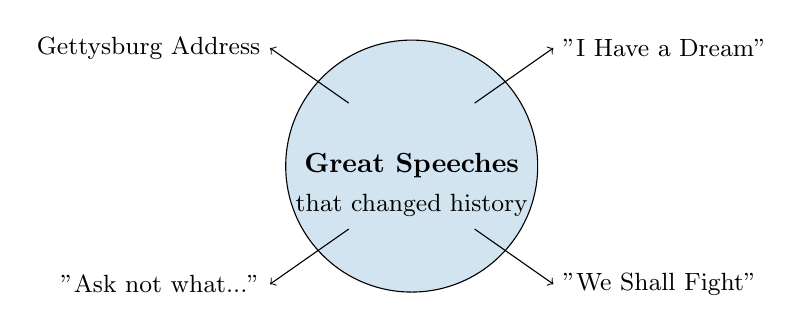
\begin{tikzpicture}
            \draw[fill=mainblue!20] (0,0) circle (1.6cm);
            \node at (0,0) {\textbf{Great Speeches}};
            \node at (0,-0.5) {\small that changed history};
            \draw[->] (0.8,0.8) -- (1.8,1.5) node[right] {\small "I Have a Dream"};
            \draw[->] (-0.8,0.8) -- (-1.8,1.5) node[left] {\small Gettysburg Address};
            \draw[->] (0.8,-0.8) -- (1.8,-1.5) node[right] {\small "We Shall Fight"};
            \draw[->] (-0.8,-0.8) -- (-1.8,-1.5) node[left] {\small "Ask not what..."};
        \end{tikzpicture}
    \end{center}
\end{frame}

% Section: Benefits
\section{Benefits of Strong Public Speaking Skills}

\begin{frame}{Professional Benefits}
    \begin{block}{Career Advancement}
        \begin{itemize}
            \item Leadership opportunities
            \item Higher visibility within organizations
            \item Ability to pitch ideas effectively
            \item Enhanced networking capabilities
        \end{itemize}
    \end{block}
    
    \begin{alertblock}{Research Shows:}
        \centering
        Professionals with strong presentation skills are \textbf{70\% more likely} to be promoted to leadership positions.
    \end{alertblock}
\end{frame}

\begin{frame}{Personal Benefits}
    \begin{columns}
        \column{0.40\textwidth}
        \begin{itemize}
            \item Increased self-confidence
            \item Better critical thinking abilities
            \item Improved interpersonal relationships
            \item Enhanced persuasion skills
        \end{itemize}
        
        \column{0.60\textwidth}
        \begin{center}
            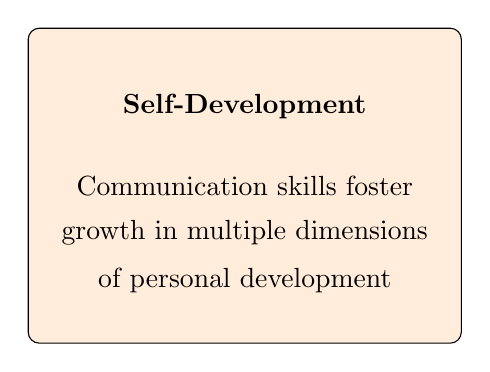
\begin{tikzpicture}
                \draw[fill=accentorange!15, rounded corners] (0,0) rectangle (5.5,4);
                \node at (2.75,3) {\textbf{Self-Development}};
                \node at (2.75,2) {Communication skills foster};
                \node at (2.75,1.4) {growth in multiple dimensions};
                \node at (2.75,0.8) {of personal development};
            \end{tikzpicture}
        \end{center}
    \end{columns}
\end{frame}

\begin{frame}{Academic Benefits}
    \begin{itemize}
        \item Improved learning through verbal articulation
        \item Better class participation and engagement
        \item Higher grades in presentation assignments
        \item Preparation for future professional requirements
    \end{itemize}
    
    \begin{center}
        \begin{tabular}{cc}
            \toprule
            \textbf{Skill} & \textbf{Impact on Academic Performance} \\
            \midrule
            Clear Articulation & 35\% improvement in comprehension \\
            Presentation Skills & 28\% higher project scores \\
            Q\&A Handling & 42\% better information retention \\
            \bottomrule
        \end{tabular}
    \end{center}
\end{frame}

% Section: Obstacles
\section{Common Obstacles}

\begin{frame}{Common Obstacles to Effective Public Speaking}
    \begin{columns}
        \column{0.6\textwidth}
        \begin{enumerate}
            \item \textbf{Fear and anxiety (glossophobia)}
                \begin{itemize}
                    \item Affects nearly 75\% of people
                \end{itemize}
            \item \textbf{Lack of preparation}
                \begin{itemize}
                    \item Content and delivery issues
                \end{itemize}
            \item \textbf{Poor structure}
                \begin{itemize}
                    \item Unclear organization of ideas
                \end{itemize}
            \item \textbf{Ineffective delivery}
                \begin{itemize}
                    \item Voice, pace, body language
                \end{itemize}
        \end{enumerate}
        
        \column{0.4\textwidth}
        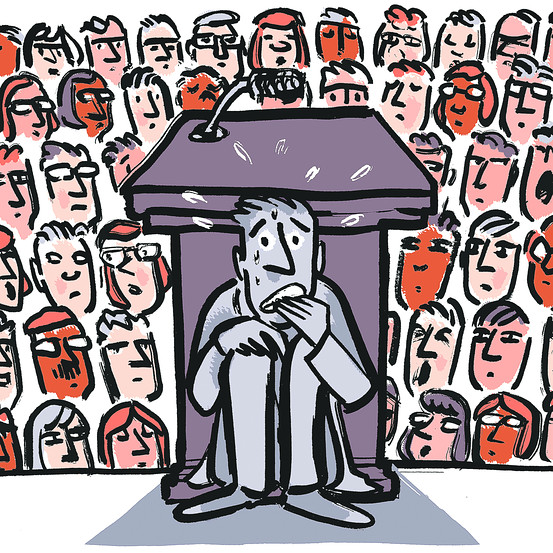
\includegraphics[width=\textwidth]{images/obstacles.jpg}
    \end{columns}
\end{frame}

% Section: Strategies
\section{Strategies to Improve}

\begin{frame}{Strategies to Improve: Preparation}
    \begin{block}{The 5P Principle}
        \begin{center}
            \textbf{Proper Preparation Prevents Poor Performance}
        \end{center}
    \end{block}
    
    \begin{itemize}
        \item \textbf{Research thoroughly}
            \begin{itemize}
                \item Know your content better than you need to
            \end{itemize}
        \item \textbf{Structure deliberately}
            \begin{itemize}
                \item Opening, body, conclusion
            \end{itemize}
        \item \textbf{Practice strategically}
            \begin{itemize}
                \item Spaced repetition, recording yourself
            \end{itemize}
        \item \textbf{Anticipate questions}
            \begin{itemize}
                \item Prepare for various scenarios
            \end{itemize}
    \end{itemize}
\end{frame}

\begin{frame}{Strategies to Improve: Technique}
    \begin{columns}
        \column{0.5\textwidth}
        \textbf{Voice Control}
        \begin{itemize}
            \item Vary pitch and tone
            \item Strategic pauses
            \item Appropriate volume
            \item Clear articulation
        \end{itemize}
        
        \textbf{Content Mastery}
        \begin{itemize}
            \item Storytelling methods
            \item Visual aids usage
            \item Metaphors \& analogies
        \end{itemize}
        
        \column{0.5\textwidth}
        \textbf{Body Language}
        \begin{itemize}
            \item Open posture
            \item Purposeful movement
            \item Engaging gestures
            \item Eye contact
        \end{itemize}
        
        \textbf{Audience Engagement}
        \begin{itemize}
            \item Interactive elements
            \item Reading the room
            \item Adapting on the fly
        \end{itemize}
    \end{columns}
\end{frame}

\begin{frame}{Professional Development Resources}
    \begin{block}{Organizations \& Communities}
        \begin{itemize}
            \item Toastmasters International
            \item Professional speaker associations
            \item University workshops and courses
            \item Corporate training programs
        \end{itemize}
    \end{block}
    
    \begin{block}{Digital Resources}
        \begin{itemize}
            \item TED Masterclass
            \item Online courses (Coursera, Udemy)
            \item Public speaking apps and simulators
            \item YouTube tutorials and channels
        \end{itemize}
    \end{block}
\end{frame}

% Section: Case Studies
\section{Case Studies}

\begin{frame}{Case Studies: Transformation Through Public Speaking}
    \begin{columns}
        \column{0.48\textwidth}
        \begin{block}{Business Leader}
            \begin{itemize}
                \item \textbf{Before:} Mid-level manager with good ideas but limited influence
                \item \textbf{Process:} Committed to weekly speaking practice
                \item \textbf{After:} Promoted to executive leadership within 18 months
            \end{itemize}
        \end{block}
        
        \column{0.48\textwidth}
        \begin{block}{Graduate Student}
            \begin{itemize}
                \item \textbf{Before:} Anxious presenter with limited academic opportunities
                \item \textbf{Process:} University speaking workshop and consistent practice
                \item \textbf{After:} Won dissertation award and multiple job offers
            \end{itemize}
        \end{block}
    \end{columns}
    
    \begin{alertblock}{Key Insight}
        \centering
        The common factor: Consistent, deliberate practice with feedback
    \end{alertblock}
\end{frame}

% Section: Action Plan
\section{Action Plan}

\begin{frame}{Action Plan: Your Path Forward}
    \begin{enumerate}
        \item \textbf{Assessment:} Evaluate your current skill level
            \begin{itemize}
                \item Self-recording, feedback from trusted peers
            \end{itemize}
        \item \textbf{Goal Setting:} Define specific targets
            \begin{itemize}
                \item Clear metrics, reasonable timeline
            \end{itemize}
        \item \textbf{Skill Development:} Focus on one aspect at a time
            \begin{itemize}
                \item Content creation $\rightarrow$ Delivery $\rightarrow$ Audience engagement
            \end{itemize}
        \item \textbf{Practical Application:} Seek opportunities
            \begin{itemize}
                \item Volunteer for presentations, join clubs
            \end{itemize}
        \item \textbf{Feedback Loop:} Continuous improvement
            \begin{itemize}
                \item Document progress, adapt strategies
            \end{itemize}
    \end{enumerate}
\end{frame}

% Section: Conclusion
\section{Conclusion}

\begin{frame}{Conclusion: The Power of Your Voice}
    \begin{block}{Key Takeaways}
        \begin{itemize}
            \item Public speaking is a fundamental life skill
            \item The benefits extend across professional, personal, and academic domains
            \item Obstacles can be systematically overcome
            \item Improvement is accessible to everyone through deliberate practice
        \end{itemize}
    \end{block}
    
    \begin{center}
        \large "Speech is power: speech is to persuade, to convert, to compel."\\
        \normalsize — Ralph Waldo Emerson
    \end{center}
\end{frame}

% Thank You slide with big centered text
\begin{frame}[plain]
    \vspace{2cm}
    \begin{center}
        \fontsize{40}{48}\selectfont\textbf{Thank You}
        
        \vspace{1.5cm}
        \normalsize Questions \& Discussion
    \end{center}
\end{frame}

\end{document}